% %%% Time-stamp: <2023-11-10 22:46:08 vladimir>
% %%% Copyright (C) 2019-2023 Vladimir G. Ivanović
% %%% Author: Vladimir G. Ivanović <vladimir@acm.org>
% %%% ORCID: https://orcid.org/0000-0002-7802-7970

\chapter{Discussion}%
\label{ch:discussion}%
\noindent\bigskip%

This chapter addresses this dissertation's research question:
\medskip%
\begin{quote}\OnehalfSpacing
  Has Rocketship structured itself to earn a return for its founders and investors, focusing especially on its real estate transactions?
\end{quote}
It looks more closely at the research question and discusses what kind of evidence would confirm or disconfirm the research question. Prior to looking at some approaches to answering the research question, it looks at three well-known approaches to making arguments for or against a proposal or policy. Then, the research question is answered and an argument is made to support that conclusion. Two final sections discuss what policy issues are raised during the examination of the data and the evidence, what further research is warranted. Lastly, this dissertation makes a brief conclusion.

\section{The Research Question}%
\label{sec:research-question}\indent%

The research question really is asking two questions:
\begin{enumerate}
  \item Has Rocketship structured itself to make money, and
  \item is real estate the vehicle that Rocketship uses to make money?
\end{enumerate}

\subsection{Types of Evidence}%
\label{sec:types-evidence}\indent%

\section{Summary and Key Findings}%
\label{sec:summary-key-findings}\indent%

\section{Approaches to Answering the Research Question}%
\label{sec:appr-answ-rese-quest}\indent%

\subsection{aRappaport's Rules}%
\label{sec:rappaports-rules}\indent%

Anatol Rapoport, a [mathematical] game theorist, proposed four rules that seek to increase understanding and avoid defensive responses. \citefirstlastauthor{Dennett2013} reformulated them in his book \citetitle{Dennett2013} \parencite{Dennett2013}:
\begin{enumerate}[topsep=0.3\baselineskip,itemsep=0.25\baselineskip]
  \item You should attempt to re-express your target’s position so clearly, vividly, and fairly that your target says, “Thanks, I wish I’d thought of putting it that way.”
  \item You should list any points of agreement (especially if they are not matters of general or widespread agreement).
  \item You should mention anything you have learned from your target.
  \item Only then are you permitted to say so much as a word of rebuttal or criticism.
\end{enumerate}
\medskip

Here, in Rocketship's case, their argument might go along the following lines:
\begin{enumerate}[topsep=0.3\baselineskip,itemsep=0.25\baselineskip]
  \item Public schools in areas of poverty, for whatever reason, don't educate children well, and they educate children of color especially poorly. We (Rocketship) aim to change this by a combination of focus, targeted intervention, and technology. We are focused on doing whatever it takes to raise the educational attainment of our students, and we focus day in and day out on this one goal. Our pedagogy has two major aspects: We monitor and target with specialize intervention students who are not doing as well as we would like, and we use technology (computer-aided instruction) to tailor instruction to a specific child's needs.

  We believe that, by controlling our facilities, we can remove a serious distraction that comes with sharing facilities with a public school district. Not only are we not beholden to the whims of the public school district, but we don't have to spend time preparing year after year a Proposition 39 facilities request. We are never embroiled in petty disputes about interactions between public school students and our students because they never arise. Our results speak for themselves. All of our schools do better than their surrounding district and do better than the California average.
  \item I agree that some public school districts have failed in their primary duty to educate children, but staying the course is not an option because doing the same thing over and over and expecting different results is not likely to be successful, now or ever.
 
  I also agree that providing separate facilities for children rather than forcing them to share is more likely to be successful than otherwise. Being able to control the teaching environment brings stability the classroom.
  \item Starting and operating a charter school is not for the faint of heart. Funding for both operation and for facilities is hard to come by, and must be procured before a single student arrives on campus. Facilities need to be constructed or modified well before classes begin. Children need to be enrolled, and parents need to be persuaded to help out. Juggling priorities, contingencies, and expectations is a full-time task, and it shows when the topics of board committee (executive, business, achievement, development) meetings are looked at.
    \item However, even given the truthfulness of the items 1–3 above, there are some areas where criticism, some of it severe, is warranted.
    \begin{itemize}[topsep=0.3\baselineskip,itemsep=0.25\baselineskip]
      \item Rocketship spends an inordinate amount of time on topics that are not academic in focus. One can see this in the topic areas of its board committees, where only one of four has to do with academic achievement.

      \item Rocketship short-changes current students in order to create future students by allocating 20\% of revenue to facilities. Although this is  legal, I suspect that the California Legislature did not one charter school begetting another and so on when they created the legislation which allowed charter schools to exist, just as they didn't anticipate the damage that for-profit charter school chains or virtual charter schools would do. 

      The percentage of revenue that Rocketship spends on administration (i.e. management), is unusually high at 15\%. Public school districts are limited to 9\%. So, right off the top, 35\% of revenue is siphoned off and does not go directly to educating children.

      \item Teachers at Rocketship schools in Santa Clara county have much less experience and are paid substantially less than, say, teachers in the San José Unified School District. If we believe that teachers are a key factor in delivering a quality education, then what kind of teachers Rocketship hires and how much it pays them are important determinants of the quality of the teaching staff and hence how well Rocketship educates its children.

      \item Rocketship has seriously exaggerated how well its students do compared to public school students. The size of the discrepancy, 4× to 5× larger than what was reported in the literature, does not bode well for Rocketship's commitment to ``eliminate the achievement gap in our lifetime.''
      
      \item Rocketship's policy of owning its facilities has led to over \$185M\footnote{This figure is for all Rocketship schools, i.e. those in  California, Tennessee, Wisconsin, Washington, D.C. and Texas.} in debt. At 3\% per annum, that's another \$5.4M that is not going directly toward educating children.
    \end{itemize}
  \end{enumerate}

\subsection{Toulmin Arguments}%
\label{sec:toulmin-arguments}\indent%

Stephen Toulmin was a British philosopher interested in moral reasoning. He developed a method for making practical arguments where ethics and morality played a role. His method has six components, of which the first three are those most commonly seen.
\begin{enumerate}[topsep=0.3\baselineskip,itemsep=0.25\baselineskip]
  \item Claims are statements, conclusions which must be justified.
  \item Evidence (facts, data) are used to provide the basis for making the claim.
  \item Warrants are the connection between the claim and the evidence which backs up the claim.
  \item Backings buttresses a warrants.
  \item Reservations are restrictions on the claim.
  \item Qualifiers express the degree of certainty about the claim.
\end{enumerate}

\prettyref{fig:toulmin-arg} below diagrams the relationship between the parts of a Toulmin argument.

\begin{figure}[ht]
  \caption{The Toulmin Argument Schema}%
  \label{fig:toulmin-arg}%
  \copyrightbox[b]{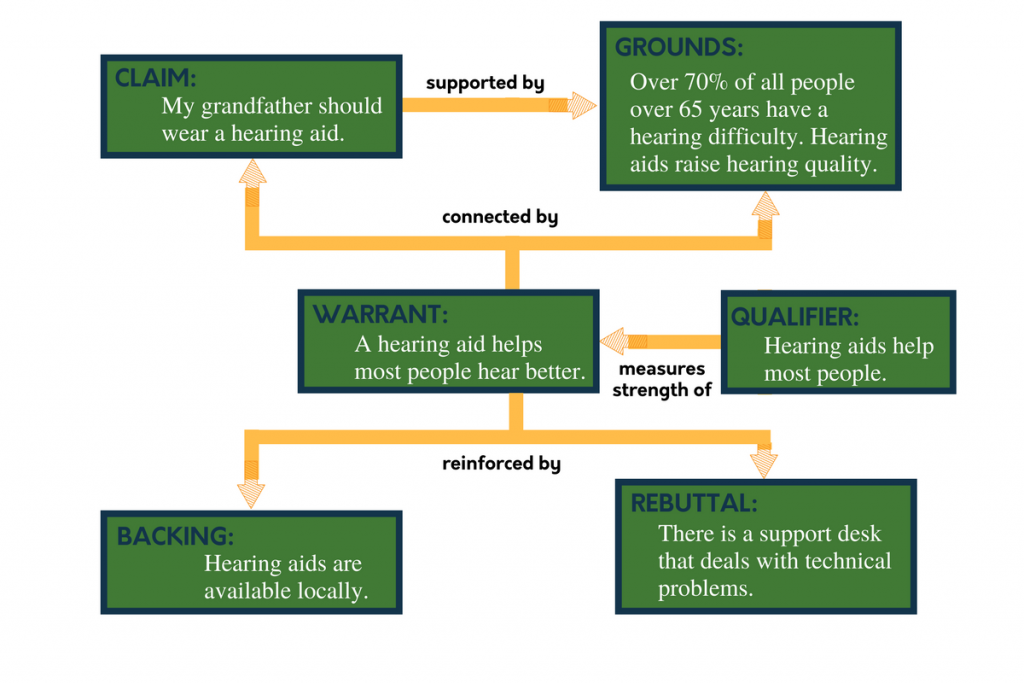
\includegraphics[scale=0.5]{The Toulmin Argument Schema}}{“Toulmin Argument,” Kalyca Schultz, Virginia Western Community College, CC-BY-SA in “Toulmin Argument Model” by Liza Long, Amy Minervini, and Joel Gladd is licensed under CC BY-NC-SA 4.0}
\end{figure}

\subsection{Logic Models}%
\label{sec:logic-models}\indent%

\section{Answering the Research Question}%
\label{sec:answ-rese-quest}\indent%

\section{Public Policy Issues}%
\label{sec:publ-policy-chang}\indent%

\section{Areas for Future Research}%
\label{sec:issu-future-rese}\indent%

\section{Conclusion}%
\label{sec:conclusion}\indent%


%%% Local Variables:
%%% mode: latex
%%% TeX-master: "Rocketship_Education-An_Exploratory_Public_Policy_Case_Study"
%%% End:
